    \chapter{ANTECEDENTES}

    \section{Orígenes de la tecnología UAV}

    Desde hace dos siglos, el espacio aéreo ha dejado de ser una frontera
    inalcanzable para integrarse plenamente, junto al dominio terrestre y marítimo, 
    como un área de proyección humana. En la actualidad, el cielo se consolida como 
    un dominio estratégico fundamental para el transporte, las comunicaciones globales 
    y la seguridad internacional. Sin embargo, y pese a lo antiintuitivo que pueda 
    parecer, el concepto de aeronave no tripulada con fines estratégico-militares se 
    remonta hasta comienzos del siglo pasado, coindiciendo con el desarrollo de la primera
    guerra mundial.

    Desde el comienzo, demostraron ser prometedoras herramientas de reconocimiento aéreo
    en las pruebas de vuelo, pero no fue hasta el estallido de la guerra de Vietnam (1946-1954)
    cuando se desplegaron a gran escala y comenzaron a usarse con diversos fines tales como actuar como señuelos en combate o lanzar misiles contra objetivos fijos entre otros. 

    Tras este conflito, muchos paises comenzaron a invertir en su desarrollo, exploración y avance tecnológico, con mnuevos modelos que mejoraban la resistencia y la capacidad de elevarse a mayor altitud. Actualmente, los drones mantienen muchos fines y aplicaciones reales, pero sin duda, su uso más conocido y relevante es el militar, en tareas de vigilancia, reconocimiento y ataques dirigidos.

    A partir de noviembre de 2013 los microdrones y los UAVs fueron 
    aprobados para su integración en el espacio aéreo de baja altitud (LAA)
    por la Administración Federal de Aviación (FAA). Esto ha provocado 
    un crecimiento muy significativo en el número de drones registrados 
    (más de 670.000 en EE. UU. en 2016 según el estudio de \cite{micro_drone_radar_studio}).Consecuentemente, surge una necesidad
    urgente de generar sistemas de legilación y regulación de estos vehículos a
        nivel nacional e internacional. 

    Sin embargo, esto deriva en varios problemas, como la dificultad de paises no desarrollados para implementar leyes y sistemas de registro tan estrictos que rigan rijan el uso de drones. Además, el tan elevado número de estos vehículos suele provocar la falta de personal de cumplimiento activo para vigilar estas leyes, así como sistemas de detección operativos y eficientes, lo cual suele dejar a la policía o fuerzas del orden sin suficientes recursos para lidiar con estas amenazas. 

    El potencial de estas tecnologías para causar daños a la seguridad pública o nacional y para cometer delitos graves (tales como la violación de la privacidad, el transporte de sustancias ilegales, colisiones inadvertidas, el despliegue de armas explosivas o agentes químicos) es enorme. El ejemplo más recurrente de el daño que estas tecnologías pueden causar es el de los peligros de colisión, donde un árticulo del IEEE en 2011 (\cite{estudio_peso_drones}) demostró que un dron de 2kg retiene la energía cinética equivalente a un proyectil antiaéreo de 20 mm (casi el doble de grande que uno de calibre 0,50).


    \section{Seguimiento de objetos individuales (SOT)}

    Dadas las numerosas problemáticas mencionadas en la anterior sección, surge la necesidad lógica de desarrollar sistemas automáticos capaces de detectar y seguir estos vehículos. Al eliminar el factor del error humano y las limitaciones ópticas, estos sistemas permiten mantener un espacio aéreo seguro, tanto en ámbitos de seguridad nacional como en la protección de la privacidad y el derecho a la intimidad, y recopilar pruebas forenses (estos sistemas pueden triangular la señal del dron para localizar al operador en caso de infracciones legales).

    Es en este contexto donde surge el concepto SOT (Single Object Traking). El seguimiento o trackeo de objetivos individuales es una tarea fundamental en el campo de la visión por computador o visión artificial (computer vision). Los sistemas SOT tienen como función rastrear un objeto concreto a lo largo de un video. El objetivo se especifica en el primer fotograma y debe ser reconocido y seguido en los fotogramas sucesivos. Esta técnica, junto con el seguimiento multi-objetivo (MOT), son las técnicas fundamentales en las aplicaciones de sistemas anti-UAVs.

    Sin embargo, como en todos los campos de investigación; los sistemas y algoritmos SOT se enfrentan a numerosos desafios y limitaciones, como los cambios repentinos de iluminación entre fotogramas, el ruido de fondo de las imágenes, la oclusión del objetivo y la escala del mismo entre otros. Debido a la presencia de estos factores en situaciones reales, los sistemas SOT deben cumplir tres características generales, según el estudio de \cite{Articulo_Concepto_SOT}: 
    \begin{itemize}
        \item \textbf{Adaptabilidad:} El sistema debe ser capaz de rastrear el objetivo incluso en condiciones adversas como ruido de fondo, oclusión o cambios de iluminación.
        \item \textbf{Robustez:} Se debe garantizar que además de las alteraciones de entorno, el sistema debe adaptarse a cambios como los movimientos complejos y repentinos del objetivo, Algo muy común en los microdrones y UAVs. Para lograr esto, el sistema debe ser capaz de detectar y rastrear las características aparentes del objetivo.
        \item \textbf{Eficiencia:} La mayoría de sistemas SOT se enfrenta a situaciones de rastreo en tiempo real, por lo que estos deben tener una alta velocidad general de procesamiento, lo que requiere implementar algoritmos de alto rendimiento.
    \end{itemize}

    \section{Clasificación de métodos SOT}

    Debido a la gran cantidad de métodos distintos que se han desarrollado desde el inicio de esta disciplina, el poco tiempo que se lleva trabajando en esta y la gran evolución que ha experimentado, actualmente no existe una clasificación estandarizada de métodos de seguimiento aceptada universalmente. Sin embargo, para este trabajo se ha optado por seguir la taxonomía propuesta por Soleimanitaleb et al. en 2022 debido a su claridad, exhaustividad y a su reciente publicación (lo que permite tener en cuenta los métodos más actuales del campo). A continuación se muestra un diagrama de esta clasificación en la figura \ref{fig:taxonomia-seguimiento-visual}.



\vspace{0.5cm}
\begin{figure}[htbp]
    \captionsetup{font=small, skip=20pt}
    \centering
    \resizebox{\textwidth}{!}{%
    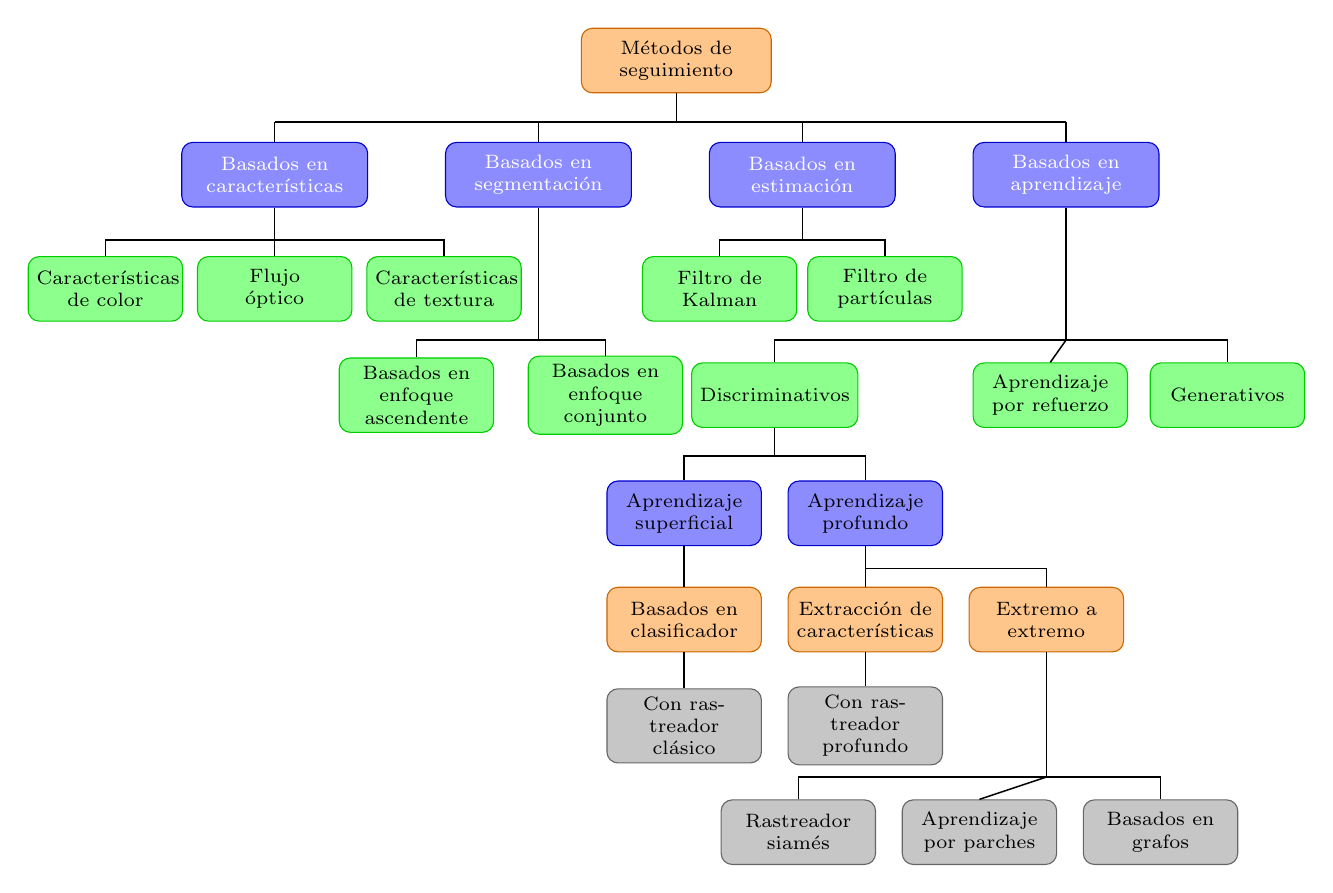
\begin{tikzpicture}[
        font=\scriptsize,
        box/.style={
            draw=#1!80!black,
            fill=#1!45,
            rounded corners=4pt,
            minimum height=0.82cm,
            align=center,
            inner sep=3pt
        },
        topbox/.style={box=orange, text width=2.2cm},
        mainbox/.style={box=blue, text=white, text width=2.15cm},
        greenbox/.style={box=green, text width=1.75cm},
        bluebox/.style={box=blue, text width=1.75cm},
        orangebox/.style={box=orange, text width=1.75cm},
        graybox/.style={box=gray, text width=1.75cm},
        line/.style={draw, line width=0.55pt}
    ]
        \node[topbox] (tracking) at (0,0) {Métodos de seguimiento};

        \node[mainbox] (feature) at (-5.1,-1.45) {Basados en\\características};
        \node[mainbox] (segmentation) at (-1.75,-1.45) {Basados en\\segmentación};
        \node[mainbox] (estimation) at (1.6,-1.45) {Basados en\\estimación};
        \node[mainbox] (learning) at (4.95,-1.45) {Basados en\\aprendizaje};

        \coordinate (topline) at (0,-0.78);
        \draw[line] (tracking.south) -- (topline);
        \draw[line] (feature |- topline) -- (learning |- topline);
        \draw[line] (feature.north) -- (feature |- topline);
        \draw[line] (segmentation.north) -- (segmentation |- topline);
        \draw[line] (estimation.north) -- (estimation |- topline);
        \draw[line] (learning.north) -- (learning |- topline);

        \node[greenbox] (color) at (-7.25,-2.9) {Características\\de color};
        \node[greenbox] (optical) at (-5.1,-2.9) {Flujo\\óptico};
        \node[greenbox] (texture) at (-2.95,-2.9) {Características\\de textura};
        \coordinate (featureline) at (-5.1,-2.28);
        \draw[line] (feature.south) -- (featureline);
        \draw[line] (color.north) |- (featureline) -| (texture.north);
        \draw[line] (optical.north) -- (featureline);

        \node[greenbox] (bottomup) at (-3.3,-4.25) {Basados en\\enfoque ascendente};
        \node[greenbox] (joint) at (-0.9,-4.25) {Basados en\\enfoque conjunto};
        \coordinate (segline) at (-1.75,-3.55);
        \draw[line] (segmentation.south) -- (segline);
        \draw[line] (bottomup.north) |- (segline) -| (joint.north);

        \node[greenbox] (kalman) at (0.55,-2.9) {Filtro de\\Kalman};
        \node[greenbox] (particle) at (2.65,-2.9) {Filtro de\\partículas};
        \coordinate (estline) at (1.6,-2.28);
        \draw[line] (estimation.south) -- (estline);
        \draw[line] (kalman.north) |- (estline) -| (particle.north);

        \node[greenbox, text width=1.9cm] (discriminative) at (1.25,-4.25) {Discriminativos};
        \node[greenbox] (reinforcement) at (4.75,-4.25) {Aprendizaje\\por refuerzo};
        \node[greenbox] (generative) at (7.0,-4.25) {Generativos};
        \coordinate (learnline) at (4.95,-3.55);
        \draw[line] (learning.south) -- (learnline);
        \draw[line] (discriminative.north) |- (learnline) -| (generative.north);
        \draw[line] (reinforcement.north) -- (learnline);

        \node[bluebox] (shallow) at (0.1,-5.75) {Aprendizaje\\superficial};
        \node[bluebox] (deep) at (2.4,-5.75) {Aprendizaje\\profundo};
        \coordinate (discline) at (1.25,-5.02);
        \draw[line] (discriminative.south) -- (discline);
        \draw[line] (shallow.north) |- (discline) -| (deep.north);

        \node[orangebox] (classifier) at (0.1,-7.1) {Basados en\\clasificador};
        \node[orangebox] (featureaction) at (2.4,-7.1) {Extracción de\\características};
        \node[orangebox] (endtoend) at (4.7,-7.1) {Extremo a\\extremo};
        \draw[line] (shallow.south) -- (classifier.north);
        \coordinate (deepline) at (2.4,-6.45);
        \draw[line] (deep.south) -- (deepline);
        \draw[line] (featureaction.north) |- (deepline) -| (endtoend.north);

        \node[graybox] (classical) at (0.1,-8.45) {Con rastreador\\clásico};
        \node[graybox] (deeptracker) at (2.4,-8.45) {Con rastreador\\profundo};
        \node[graybox] (siamese) at (1.55,-9.8) {Rastreador\\siamés};
        \node[graybox] (patch) at (3.85,-9.8) {Aprendizaje\\por parches};
        \node[graybox] (graph) at (6.15,-9.8) {Basados en\\grafos};

        \draw[line] (classifier.south) -- (classical.north);
        \draw[line] (featureaction.south) -- (deeptracker.north);
        \coordinate (endline) at (4.7,-9.1);
        \draw[line] (endtoend.south) -- (4.7,-9.1);
        \draw[line] (siamese.north) |- (endline) -| (graph.north);
        \draw[line] (patch.north) -- (endline);
    \end{tikzpicture}%
    }
    \caption[Taxonomía de métodos de seguimiento visual]{Taxonomía de métodos de seguimiento visual, \cite{Articulo_Concepto_SOT}.}
    \label{fig:taxonomia-seguimiento-visual}
\end{figure}

    \subsection{Métodos basados en características}
    Esta familia de métodos suelen ser la vía más fácil y directa para abordar el prolema del seguimiento de objetos. Se basan en una extracción previa de propiedades del objetivo como el color, la textura o el flujo óptico para rastrearlo a lo largo de la secuencia de imágenes. Estas propiedades deben ser únicas para poder ser diferenciadas de otros objetos o del fondo de la imagen, actuando como signo de identidad del objetivo. Una vez se extraen estas características, se usan para encontrar el objeto más similar al objetivo en el siguiente frame siguiendo algún criterio de similitud, repitiéndose este proceso para cada frame de la secuencia. 

    \subsection{Imágenes térmicas en el espectro infrarrojo}

    Uno de los principales retos a los que se enfrentan los sistemas de seguimiento de UAVs es la condición del entorno. Un buen sistema SOT debe poder detectar y seguir objetivos en cualquier momento del día y bajo cualquier condición adversa (temperatura, humedad, temporal...), lo cual es especialmente complicado en las horas nocturnas o de poca luz natural, y en entornos con niebla, lluvia, rachas fuertes de viento y demás fenómenos ambientales. Estos factores no solo reducen a menudo la calidad de la imagen, sino que además introducen ruido y variaciones en la firma del objetivo. Es por esto que la tecnología de imágenes infrarrojas comenzó a ser muy relevante en este campo.

    La tecnología de procesado de ímagenes térmicas en el espectro infrarrojo (TIR) consiste en la reconstrucción de imágenes a través de la radiación infrarroja emitida por los objetos de la escena. Una de las principales ventajas de este proceso es su capacidad para no interferir directamente con el objetivo, ya que la radiación electromagnética es una propiedad física inherente a cualquier cuerpo con una temperatura por encima del cero absoluto. Al limitarse a recibir dicha señal sin emitir energía externa, los detectores TIR se clasifican como sistemas de detecciñón pasivos, lo que los hace ideales para aplicaciones militares y de vigilancia. 

    Pese a todas sus ventajas, el proceso de obtención de estas imágenes requiere una serie de etapas de procesamiento debido al bajo contraste y a la escasa resolución de los detalles de la imagen. Estas etapas de procesamiento suelen llevarse a cabo a través técnicas de visión artificial (computer vision) y aprendizaje profundo (deep learning) \cite{review_infrared_imaging}.


